\documentclass{article}

\makeatletter
\def\input@path{{reports/}{./}}
\makeatother

\usepackage[preprint]{neurips_2024}
\usepackage[UTF8]{ctex}
\usepackage{amsmath}
\usepackage{booktabs}
\usepackage{graphicx}
\usepackage{subcaption}
\usepackage{array}
\graphicspath{{reports/figures/}{figures/}}
\usepackage{hyperref}
\usepackage[numbers]{natbib}

\title{HW3: Multi-Source 3D Asset Fusion and ACT Generalization on CALVIN}

\author{%
  Team HW3-DL-Spatial-Intelligence\\
  Deep Learning and Spatial Intelligence\\
  \texttt{https://github.com/Zhuyy66/HW3-DL-Spatial-Intelligence}
}

\begin{document}

\maketitle

\begin{abstract}
本报告完成课程作业 HW3 的两条主线：Topic 1 构建多来源 3D 资产并融合到真实背景场景，Topic 2 训练 ACT 策略并评估其在 CALVIN 未见环境中的泛化能力。Topic 1 以 Mip-NeRF 360 \texttt{counter} 场景为背景，分别使用真实多视角重建、DreamFusion text-to-3D 和 Stable Zero123 image-to-3D 生成 \texttt{object\_A}、object B hamburger 和 object C toy，再通过 Blender 统一坐标、尺度、材质和相机轨迹，输出 300 帧融合视频与关键帧。Topic 2 基于官方 \texttt{xiaoma26/calvin-lerobot} splits，在 splitA 上训练 A-only ACT，在 splitA/B/C 上训练 ABC ACT，并在未见 splitD 上计算 open-loop Action L1。结果显示，ABC 在 splitD normalized Action L1 上从 A-only 的 0.6586 降至 0.5780，相对降低 12.24\%，且 frame-level p95 误差降低 8.45\%。这些结果说明，多环境训练能提升跨环境动作预测鲁棒性；同时，Topic 1 的融合实验揭示了跨表示 3D 资产在纹理、尺度和渲染管线对齐上的工程挑战。
\end{abstract}

\section{Introduction}

本作业围绕空间智能中的两个互补问题展开。Topic 1 关注 3D 内容生成与真实场景融合：给定真实背景、真实采集物体、文本提示物体和单图物体，目标是把来源、表示形式和质量特征各不相同的资产放入同一世界坐标系，并输出可复现的多视角融合视频。Topic 2 关注机器人模仿学习：在 CALVIN 桌面操作数据集上训练 Action Chunking Transformer (ACT)，并检验单环境训练与多环境训练在未见环境 D 上的泛化差异。

两条主线共享同一个工程准则：所有结论必须能追溯到明确的数据、脚本、日志和可复现文件。对于 3D 融合，资产来自 3D Gaussian Splatting (3DGS)、DreamFusion 和 Stable Zero123；这些方法的输入成本、几何一致性、纹理质量和导出形式各不相同。仅获得单个可视化结果并不足够，报告还需要说明如何把 Gaussian、mesh、texture 和 camera path 统一成一个可渲染场景。对于机器人学习，ACT 的效果会受到 dataset split、训练预算、动作归一化、chunk size、图像预处理和评测环境的共同影响。为避免不公平比较，A-only 与 ABC 模型使用相同结构、相同 150000 gradient steps、相同 batch size、相同 optimizer 和相同随机种子，主要差异限定为训练数据覆盖范围。

本报告的交付物包括三类内容。第一，Topic 1 提供 \texttt{counter} 背景、\texttt{object\_A}、object B 和 object C 的图表证据，包含 render-vs-GT contact sheet、生成结果、导出纹理、counter orbit 帧与融合视频关键帧。第二，Topic 2 提供 A-only 与 ABC 的训练曲线、splitD Action L1 对比、per-chunk 误差曲线和 frame-level 误差分布。第三，仓库保存可复现实验入口、轻量结果 JSON/CSV/MD、报告图表和外部大文件 manifest；大体积 checkpoint、mesh、video 和 raw dataset 保持在 Git 外部。

\section{Related Work}

多视角重建为真实场景融合提供几何基础。COLMAP 通过 Structure-from-Motion 和 Multi-View Stereo 估计相机位姿、稀疏点云与稠密几何，是许多神经渲染方法的前置步骤\cite{schonberger2016sfm,schonberger2016mvs}。3D Gaussian Splatting 使用可微的各向异性 Gaussian 表示场景，在高质量新视角合成与实时渲染之间取得较好平衡\cite{kerbl2023gaussian}。本作业中的 \texttt{counter} 背景和 \texttt{object\_A} 先采用 3DGS 获得稳定的新视角渲染，再通过 textured mesh 或 pass-level 合成接入最终融合流程。

文本或单图驱动的 3D 生成扩展了资产来源。DreamFusion 使用预训练 text-to-image diffusion model 提供 score distillation signal，从文本提示优化 3D 表示\cite{poole2022dreamfusion}。Zero-1-to-3 学习单张图像到新视角图像的生成先验，为 image-to-3D 优化提供条件视图监督\cite{liu2023zero123}；Stable Zero123 与 threestudio 将这些方法整理成可运行的开源管线\cite{stability2023zero123,threestudio2023}。这类方法降低了采集成本，但在局部几何、纹理漂移、尺度控制和 mesh 清理上仍需要人工审计。

机器人模仿学习部分基于 CALVIN 和 ACT。CALVIN 提供跨桌面环境的语言条件长时程操作任务，可用于评估策略在不同视觉布局和物体配置下的泛化能力\cite{mees2022calvin}。ACT 通过 Transformer 预测未来一段动作 chunk，降低逐步控制中的高频查询压力，并提升长时程操作的稳定性\cite{chi2023act}。LeRobot 提供统一 dataset schema、policy config 和训练入口\cite{lerobot2024}，便于从 offline demonstrations 构造可重复训练与评测流程。本作业在 LeRobot 训练侧与 CALVIN 评测侧之间建立双环境桥接，并以 splitD open-loop Action L1 作为主要可比指标。

\section{Datasets}

\subsection{CALVIN Official Splits}

Topic 2 使用课程指定的官方 \texttt{xiaoma26/calvin-lerobot} 数据。该数据来自 CALVIN 语言条件桌面操作基准，包含 Franka Panda 机械臂在四个环境中的演示轨迹。每条样本包含 15 维状态、7 维相对末端动作、静态相机图像、腕部相机图像、episode index 和 task index。训练侧使用 Python 3.12 与 LeRobot 0.4.0，评测侧保留 CALVIN 官方 Python 3.8 环境，因此数据进入训练前会转换为 LeRobot canonical keys：\texttt{observation.state}、\texttt{action}、\texttt{observation.images.image} 和 \texttt{observation.images.wrist\_image}。

表~\ref{tab:calvin-splits} 给出官方 split 统计。splitA 用于 A-only 训练，splitA/B/C 合并后用于 ABC 训练，splitD 作为未见环境评测集合。早期数据审计曾通过修正版 \texttt{scene\_info.npy} 和 \texttt{episodes\_stats.original\_frame\_idx} 反推环境标签，并与官方 A/B/C episode 数完全对齐；正式报告口径以官方 split 为准，旧审计只作为数据划分可追溯性的辅助证据。

\begin{table}[h]
  \centering
  \caption{CALVIN official split statistics used in Topic 2.}
  \label{tab:calvin-splits}
  \begin{tabular}{llrr}
    \toprule
    Split & Scene & Episodes & Frames \\
    \midrule
    splitA & A & 6089 & 366693 \\
    splitB & B & 6115 & 367096 \\
    splitC & C & 5666 & 337954 \\
    splitD & D & 5124 & 308918 \\
    \bottomrule
  \end{tabular}
\end{table}

ABC 联合训练使用单个 LeRobot v3 canonical dataset。由于 splitA、splitB 和 splitC 的 \texttt{episode\_index} 均从 0 开始，项目先构建 \texttt{abc\_joint\_canonical\_v3}，把三组 episode 重映射到连续区间 \texttt{0..17869}，并通过 \texttt{source\_task\_index -> task string -> canonical\_task\_index} 对齐任务命名空间。最终 ABC 数据包含 17870 条 episode、1071743 帧和 89 个任务，并通过 \texttt{abc\_remap\_manifest.jsonl} 与 schema repair summary 记录来源 split、原始 episode、任务字符串、重映射索引和长度。

\subsection{3D Fusion Assets}

Topic 1 的背景选择 Mip-NeRF 360 \texttt{counter}。该场景包含真实厨房台面图像和 COLMAP 相机参数，桌面尺度适合放置 object A/B/C，也与 hamburger 等生成式资产的语义一致。项目对 \texttt{counter} 运行 3DGS 7k smoke training 与 30k full training，并导出 orbit camera path 与 textured mesh，作为最终 Blender 融合的世界坐标基准。

\texttt{object\_A} 来自手机环绕视频采集。视频经过抽帧、COLMAP 注册、3DGS 训练和 mesh/texturing 后，成为真实多视角重建路线的代表。该路线的优点是几何和纹理直接来自真实观测，质量主要受拍摄轨迹、特征匹配、点云清理和纹理重建影响。object B 采用 threestudio / DreamFusion 路线，prompt 为 ``a hamburger''，完整训练 10000 iterations 并导出 \texttt{obj+mtl+texture}。object C 采用 Stable Zero123 路线，以主体居中的 RGBA 图像作为输入，最终选择 3000-iteration 导出版本作为报告主展示。B/C 均以 textured mesh 形式进入 Blender。

\section{Methods}

\subsection{Topic 1: Multi-Source 3D Asset Fusion}

Topic 1 的流程分为四步。第一步，真实背景 \texttt{counter} 和真实物体 \texttt{object\_A} 使用 COLMAP + 3DGS 获得新视角渲染能力，并进一步通过 dense meshing 与 texture reconstruction 获得 Blender 可读 mesh。第二步，object B 通过 DreamFusion text-to-3D 生成 hamburger mesh；该路线先用 100-step smoke run 验证 SDS 优化链路，再运行 10000-step full run 并导出纹理文件。第三步，object C 通过 Stable Zero123 image-to-3D 生成 toy mesh；项目比较 3000 与 10000 iterations 的可视效果后选择 3000 版本作为稳定展示。第四步，所有资产导入 Blender，在 \texttt{counter} 坐标系下统一尺度、朝向、位置、材质和相机轨迹，输出 300 帧、30 fps、3114$\times$2076 的融合视频。

跨表示统一是 Topic 1 的核心工程点。3DGS 适合高质量新视角渲染，mesh 适合在 Blender 中统一摆放和材质管理。为降低工具链割裂，项目保留两种策略：可 mesh 化的资产进入 Blender 统一渲染；对仍保留 Gaussian 表示的资产，可使用同轨迹双 pass 渲染与 alpha 合成。最终报告主结果采用 Blender 中的 textured mesh 组合，配合从 \texttt{counter} 相机集合采样得到的 300 帧 orbit trajectory。

\subsection{Topic 2: ACT/CALVIN Cross-Environment Generalization}

Topic 2 采用 ACT 作为模仿学习策略。ACT 以当前视觉观测和机器人状态为输入，使用 Transformer encoder-decoder 预测未来动作 chunk。项目配置使用 \texttt{chunk\_size=100} 与 \texttt{n\_action\_steps=100}，动作维度为 7；前 6 维表示相对末端位姿增量，最后 1 维表示夹爪命令。训练时模型对完整 future action chunk 计算 L1 loss，并使用 \texttt{action\_is\_pad} 屏蔽 episode 末尾越界动作。

训练入口由 \texttt{topic2\_act/scripts/run\_act\_train.py} 封装。A-only 只使用 splitA，ABC 使用 splitA/B/C 的合并 canonical dataset。两组训练共享 ACT 结构、ResNet18 ImageNet backbone、batch size、learning rate、weight decay、seed、DataLoader 配置和 150000 gradient steps。评测主要使用 splitD open-loop Action L1：脚本直接读取 splitD raw parquet，构造与训练一致的 100-step future action chunk，加载 checkpoint 的 preprocessor 与 policy，并在 normalized action space 与 raw action units 中计算有效动作元素的平均 L1。

CALVIN closed-loop rollout 依赖 PyBullet/EGL 图形栈。由于服务器 strict NVIDIA EGL 路线在最终检查中仍受 GLVND/NVIDIA userspace 限制，报告将全量 splitD open-loop Action L1 作为主指标，把 \texttt{direct-cameras} closed-loop smoke 作为辅助证据。双环境桥接中，CALVIN Python 3.8 进程负责 \texttt{reset()} 与 \texttt{step(obs, goal)}，LeRobot Python 3.12 worker 负责图像缩放、状态整理、normalization、ACT 推理和 action queue。跨进程通信返回纯 Python \texttt{list[float]}，避免 Python/NumPy 跨版本 pickle 兼容问题。

\section{Experiments}

\subsection{Topic 1: 3D Reconstruction, Generation, and Fusion}

Topic 1 的 3DGS 结果见表~\ref{tab:topic1-psnr}。背景 \texttt{counter} 的 30k 模型达到 test PSNR 29.2630，\texttt{object\_A} 的 30k 模型达到 test PSNR 31.3322。图~\ref{fig:topic1-contact} 给出两者的 render-vs-GT contact sheet，说明真实背景和真实采集物体的重建链路均已获得可用的新视角渲染质量。

\begin{table}[h]
  \centering
  \caption{Topic 1 3DGS reconstruction metrics.}
  \label{tab:topic1-psnr}
  \begin{tabular}{lrrr}
    \toprule
    Asset & Iteration & Test PSNR & Train PSNR \\
    \midrule
    \texttt{counter} & 7000 & 27.3455 & 28.9319 \\
    \texttt{counter} & 30000 & 29.2630 & 31.5692 \\
    \texttt{object\_A} & 7000 & 31.1154 & 34.7399 \\
    \texttt{object\_A} & 30000 & 31.3322 & 37.7307 \\
    \bottomrule
  \end{tabular}
\end{table}

\begin{figure}[h]
  \centering
  \begin{subfigure}{0.48\linewidth}
    \centering
    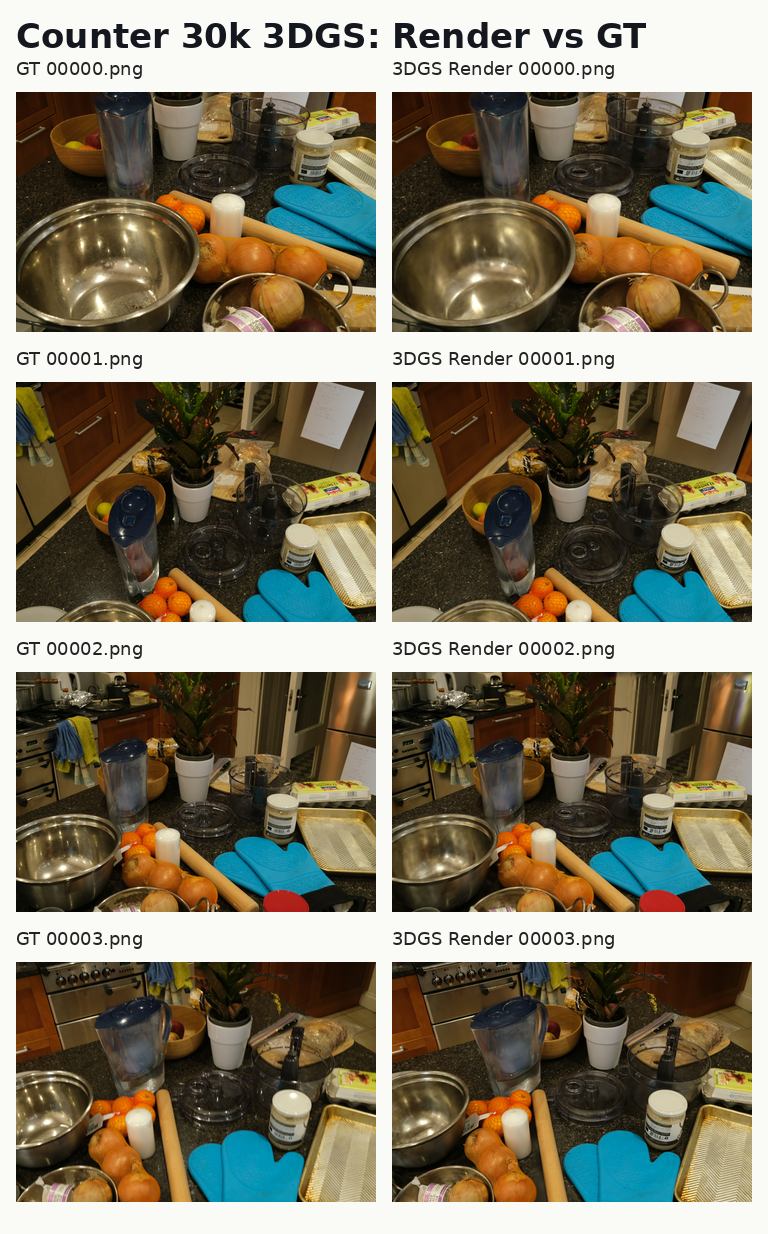
\includegraphics[width=\linewidth]{final_report/counter_30k_render_gt_contact_sheet.png}
    \caption{\texttt{counter} 30k}
  \end{subfigure}
  \begin{subfigure}{0.48\linewidth}
    \centering
    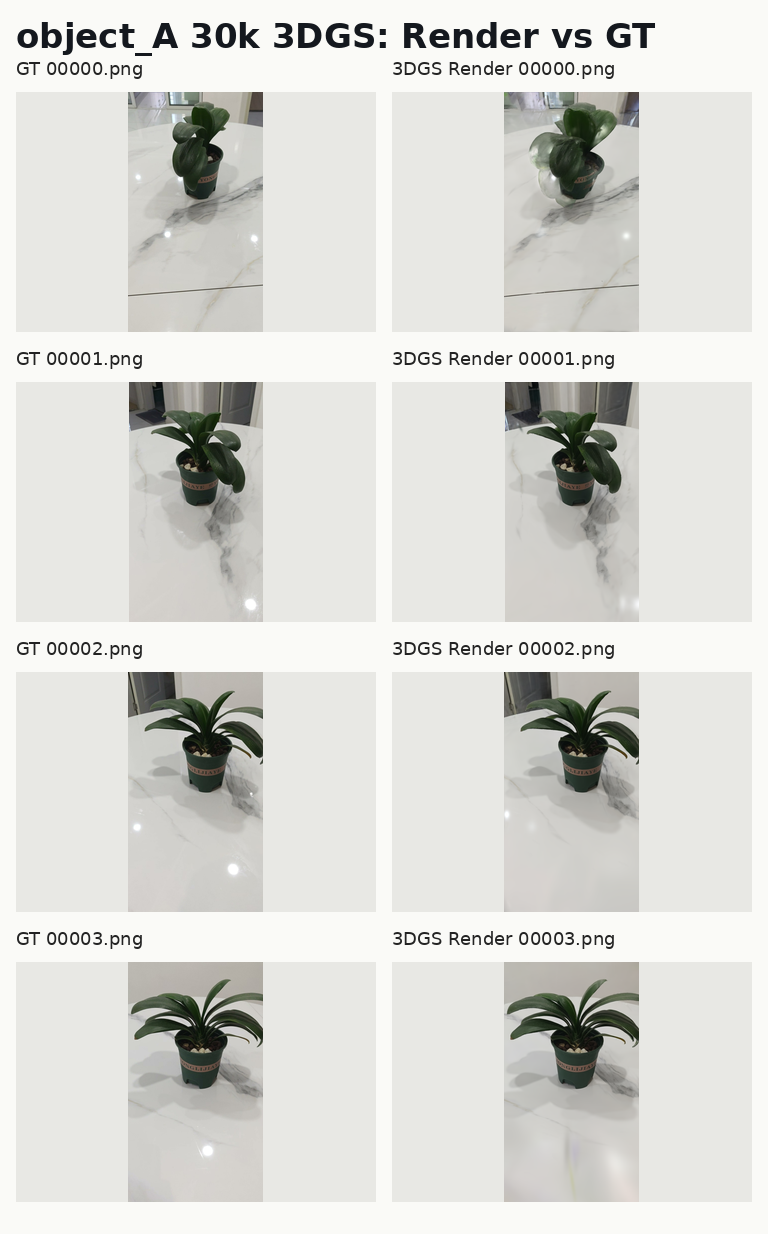
\includegraphics[width=\linewidth]{final_report/object_A_30k_render_gt_contact_sheet.png}
    \caption{\texttt{object\_A} 30k}
  \end{subfigure}
  \caption{Render-vs-GT contact sheets for the real background and real captured object.}
  \label{fig:topic1-contact}
\end{figure}

生成式资产结果见图~\ref{fig:topic1-generated-assets}。object B hamburger 使用 DreamFusion + SD 1.5，完成 100-step smoke 和 10000-step full run，报告采用 10000-step validation 与导出纹理。object C toy 使用 Stable Zero123，完成 3000 与 10000 iterations 对照，报告采用 3000-step 导出版本，因为该版本在轮廓稳定性与纹理可用性之间更均衡。

\begin{figure}[h]
  \centering
  \begin{subfigure}{0.24\linewidth}
    \centering
    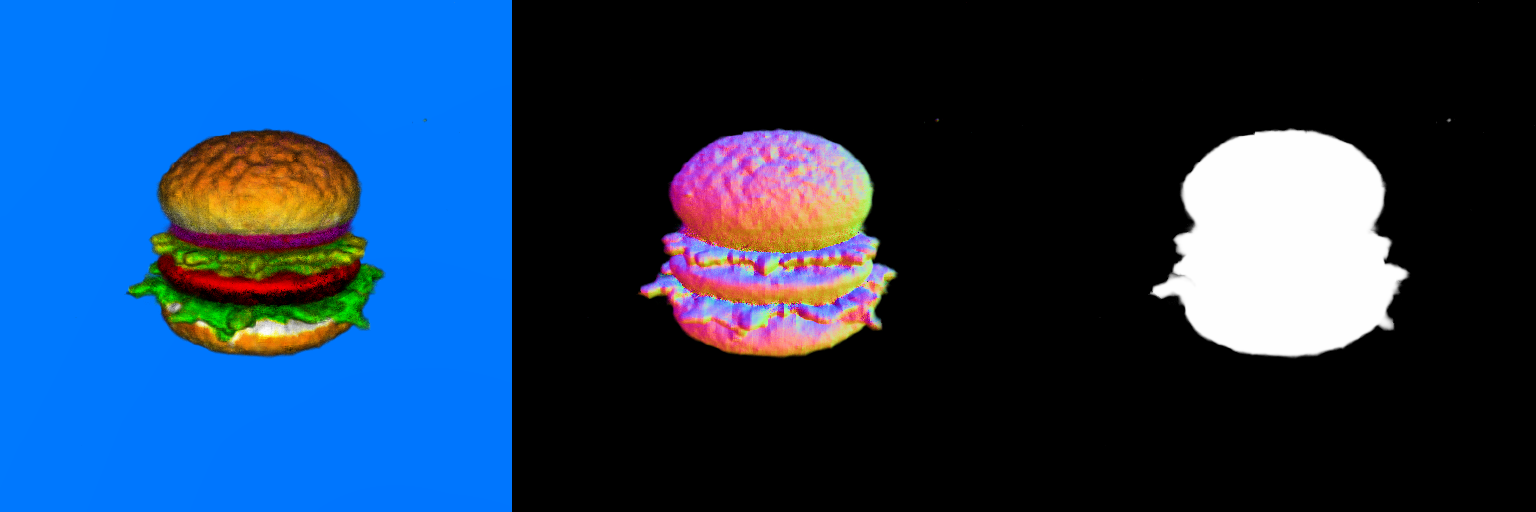
\includegraphics[width=\linewidth]{final_report/hamburger_it10000_validation.png}
    \caption{object B validation}
  \end{subfigure}
  \begin{subfigure}{0.24\linewidth}
    \centering
    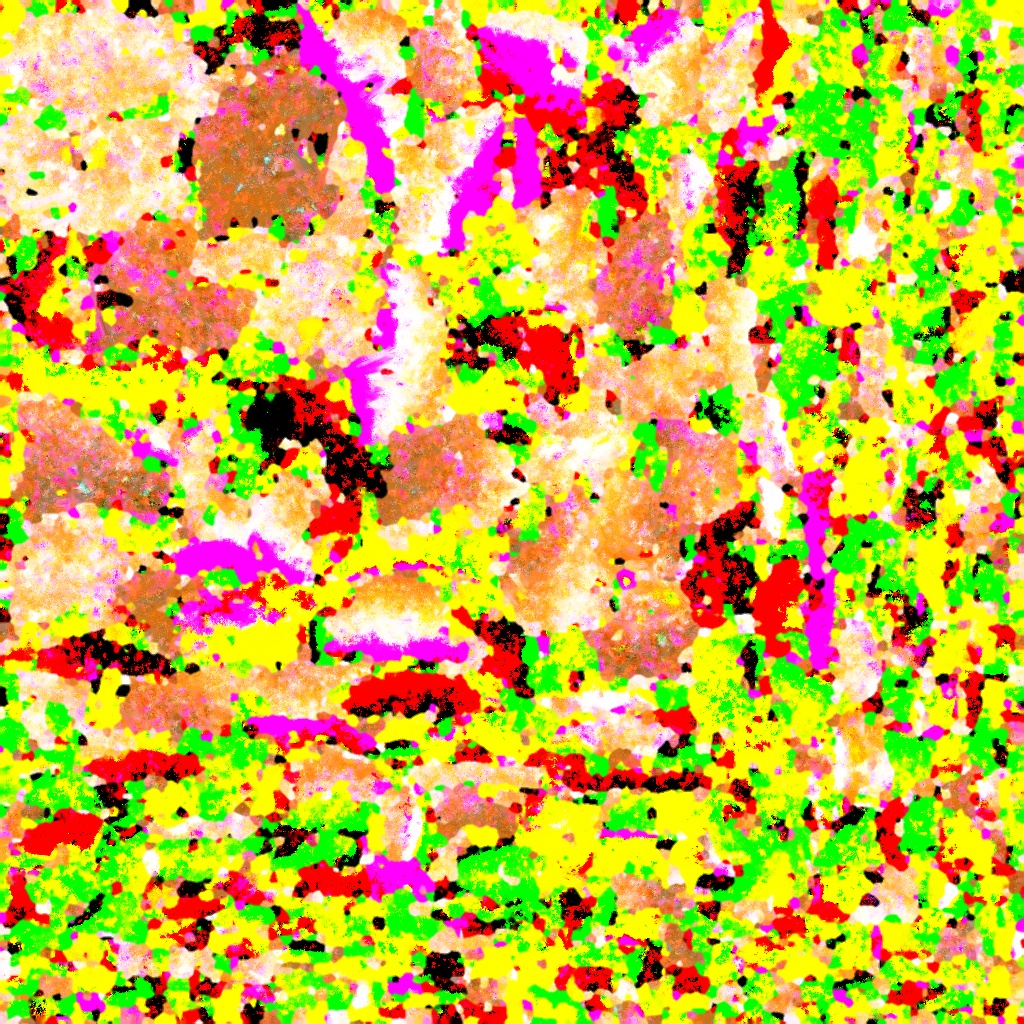
\includegraphics[width=\linewidth]{final_report/hamburger_texture_kd.jpg}
    \caption{object B texture}
  \end{subfigure}
  \begin{subfigure}{0.24\linewidth}
    \centering
    
\includegraphics[width=\linewidth]{final_report/objectC_training_strip.png}
    \caption{object C strip}
  \end{subfigure}
  \begin{subfigure}{0.24\linewidth}
    \centering
    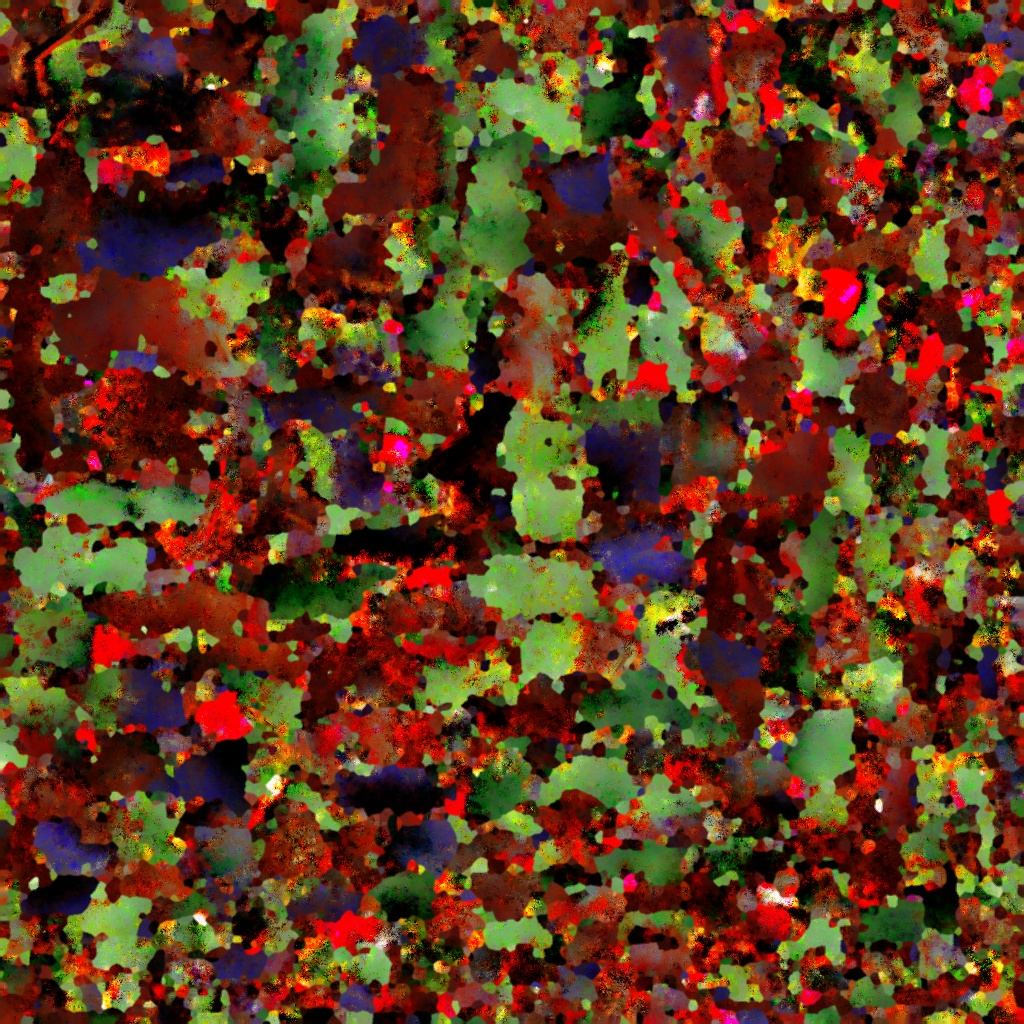
\includegraphics[width=\linewidth]{final_report/objectC_texture_kd.jpg}
    \caption{object C texture}
  \end{subfigure}
  \caption{Generated Topic 1 assets used in the final fusion scene.}
  \label{fig:topic1-generated-assets}
\end{figure}

表~\ref{tab:topic1-three-way} 总结三种资产来源的差异。真实多视角重建在几何真实性和可度量指标上最强；text-to-3D 的语义自由度最高；single-image-to-3D 的采集成本最低，但更依赖输入图像分割和透明背景质量。

\begin{table}[h]
  \centering
  \caption{Topic 1 three-way asset generation comparison.}
  \label{tab:topic1-three-way}
  \resizebox{\linewidth}{!}{%
    \begin{tabular}{lllll}
      \toprule
      Route & Asset & Strength & Main limitation & Final form \\
      \midrule
      Real multi-view reconstruction & \texttt{object\_A} & Best physical consistency; test PSNR 31.3322 & Requires capture, COLMAP, cleanup, meshing, texturing & 3DGS + textured mesh \\
      Text-to-3D & object B hamburger & High semantic freedom from prompt & SDS blur and prompt/seed sensitivity & Textured mesh \\
      Single-image-to-3D & object C toy & Lowest data cost from one RGBA image & Sensitive to crop, alpha matte, and view prior & 3000-step textured mesh \\
      \bottomrule
    \end{tabular}%
  }
\end{table}

图~\ref{fig:topic1-orbit} 展示 \texttt{counter} orbit camera path 的 Blender 验证帧；图~\ref{fig:topic1-fusion-keyframes} 展示最终融合视频的三张报告关键帧。三张关键帧均能看到 \texttt{counter} 背景、真实重建物体 A、DreamFusion hamburger 和 Stable Zero123 toy 在同一相机轨迹下的空间关系。完整视频路径记录在 \path{reports/topic1_delivery_2026-06-22/docs/external_artifacts_manifest.md}。

\begin{figure}[h]
  \centering
  \begin{subfigure}{0.48\linewidth}
    \centering
    \includegraphics[width=\linewidth]{final_report/counter_orbit_frame_0000.png}
    \caption{orbit frame 0000}
  \end{subfigure}
  \begin{subfigure}{0.48\linewidth}
    \centering
    \includegraphics[width=\linewidth]{final_report/counter_orbit_frame_0075.png}
    \caption{orbit frame 0075}
  \end{subfigure}
  \caption{Counter orbit frames used to verify the shared Blender camera path.}
  \label{fig:topic1-orbit}
\end{figure}

\begin{figure}[h]
  \centering
  \begin{subfigure}{0.32\linewidth}
    \centering
    \includegraphics[width=\linewidth]{final_report/fusion_frame_0075.png}
    \caption{frame 0075}
  \end{subfigure}
  \begin{subfigure}{0.32\linewidth}
    \centering
    \includegraphics[width=\linewidth]{final_report/fusion_frame_0150.png}
    \caption{frame 0150}
  \end{subfigure}
  \begin{subfigure}{0.32\linewidth}
    \centering
    \includegraphics[width=\linewidth]{final_report/fusion_frame_0225.png}
    \caption{frame 0225}
  \end{subfigure}
  \caption{Selected final fusion keyframes from the 300-frame Topic 1 video.}
  \label{fig:topic1-fusion-keyframes}
\end{figure}

\subsection{Topic 2: ACT Training and CALVIN Rollout}

Topic 2 的正式比较使用相同 ACT 结构和相同 150000 gradient steps。A-only 使用 splitA 训练，ABC 使用 splitA/B/C 训练；两者共享网络结构、优化器、随机种子、动作分块长度和 DataLoader 配置，完整超参见表~\ref{tab:topic2-hyperparams}。训练过程中的 action L1 曲线见图~\ref{fig:topic2-train-action-l1}。A-only 最终训练 action L1 为 0.0813，ABC 最终训练 action L1 为 0.1567；该数值用于说明训练收敛状态，最终泛化结论以 splitD 离线评测为准。

\begin{table}[h]
  \centering
  \caption{Topic 2 ACT architecture, data, and training hyperparameters.}
  \label{tab:topic2-hyperparams}
  \resizebox{\linewidth}{!}{%
    \begin{tabular}{llll}
      \toprule
      Group & Setting & Value & Source \\
      \midrule
      Model & Policy / backbone & ACT / ResNet18 ImageNet & \texttt{act\_calvin\_week3\_150k.yaml}; default dump \\
      Transformer & Dim / heads / layers & 512 / 8 / encoder 4, decoder 1 & ACT default dump \\
      VAE and loss & Latent / KL / dropout & 32 / 10.0 / 0.1 & ACT default dump \\
      Observations & State / action dims & 15 / 7 & \texttt{act\_calvin\_week3\_150k.yaml} \\
      Images & Static / wrist shapes & $200{\times}200{\times}3$ / $84{\times}84{\times}3$ & \texttt{act\_calvin\_week3\_150k.yaml} \\
      Chunking & \texttt{chunk\_size} / \texttt{n\_action\_steps} & 100 / 100 & \texttt{act\_calvin\_week3\_150k.yaml} \\
      A-only data & Episodes / frames & 6089 / 366693 & A-only \texttt{run\_manifest.json} \\
      ABC data & Episodes / frames & 17870 / 1071743 & ABC \texttt{run\_manifest.json} \\
      Optimizer & Type / lr / weight decay & AdamW / $10^{-5}$ / $10^{-4}$ & \texttt{act\_calvin\_week3\_150k.yaml} \\
      Budget & Batch / steps / seed & 8 / 150000 / 20260529 & manifests; config yaml \\
      Loader & Workers / prefetch / persistent & 16 / 4 / true & manifests \\
      Logging & WandB runs & \texttt{cnfwf30s} / \texttt{eysfzlqn} & A-only / ABC manifests \\
      \bottomrule
    \end{tabular}%
  }
\end{table}

\begin{figure}[h]
  \centering
  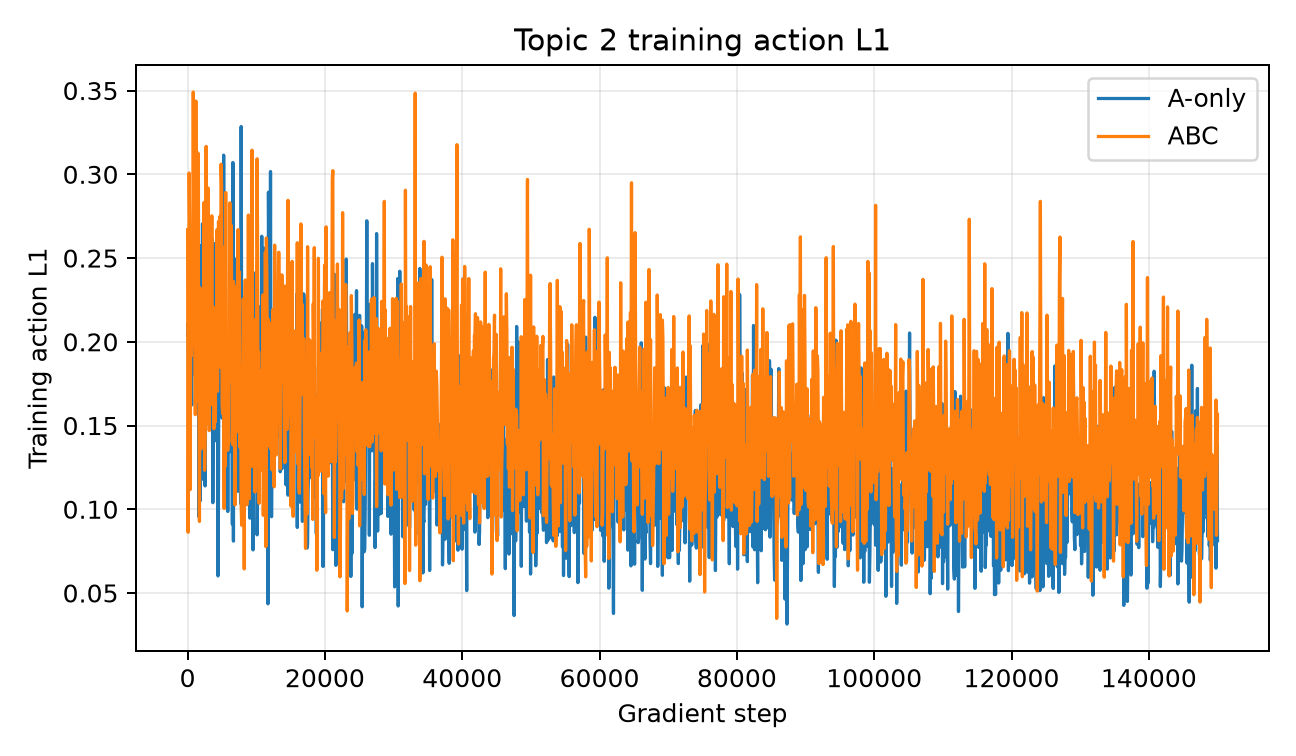
\includegraphics[width=0.82\linewidth]{topic2_train_action_l1_curve.png}
  \caption{Training action L1 curves for the comparable-budget A-only and ABC ACT runs.}
  \label{fig:topic2-train-action-l1}
\end{figure}

环境 D zero-shot 主指标采用 open-loop Action L1。评测脚本覆盖 5124 条 episode 和 308918 帧，构造与 ACT 训练一致的 100 步 future action chunk，并在有效动作元素上计算平均 L1。表~\ref{tab:topic2-d-l1} 给出完整比较。ABC 在 normalized action space 中从 0.6586 降至 0.5780，相对降低 12.24\%；raw action units 从 0.1934 降至 0.1687，相对降低 12.76\%。

\begin{table}[h]
  \centering
  \caption{A-only vs ABC on environment D open-loop Action L1. Lower is better.}
  \label{tab:topic2-d-l1}
  \resizebox{\linewidth}{!}{%
    \begin{tabular}{llrrrrll}
      \toprule
      Model & Training data & Steps & D norm. L1 & D raw L1 & Frame p95 & Closed-loop & Source result \\
      \midrule
      A-only & splitA & 150000 & 0.658629 & 0.193360 & 1.062686 & Smoke only & \texttt{a\_only\_splitD\_action\_l1\_day6\_distribution.json} \\
      ABC & splitA+splitB+splitC & 150000 & 0.577993 & 0.168696 & 0.972841 & Smoke only & \texttt{abc\_splitD\_action\_l1\_day6\_distribution.json} \\
      ABC rel. reduction & vs A-only & -- & 12.24\% & 12.76\% & 8.45\% & -- & \texttt{day6\_action\_chunking\_robustness.json} \\
      \bottomrule
    \end{tabular}%
  }
\end{table}

\begin{figure}[h]
  \centering
  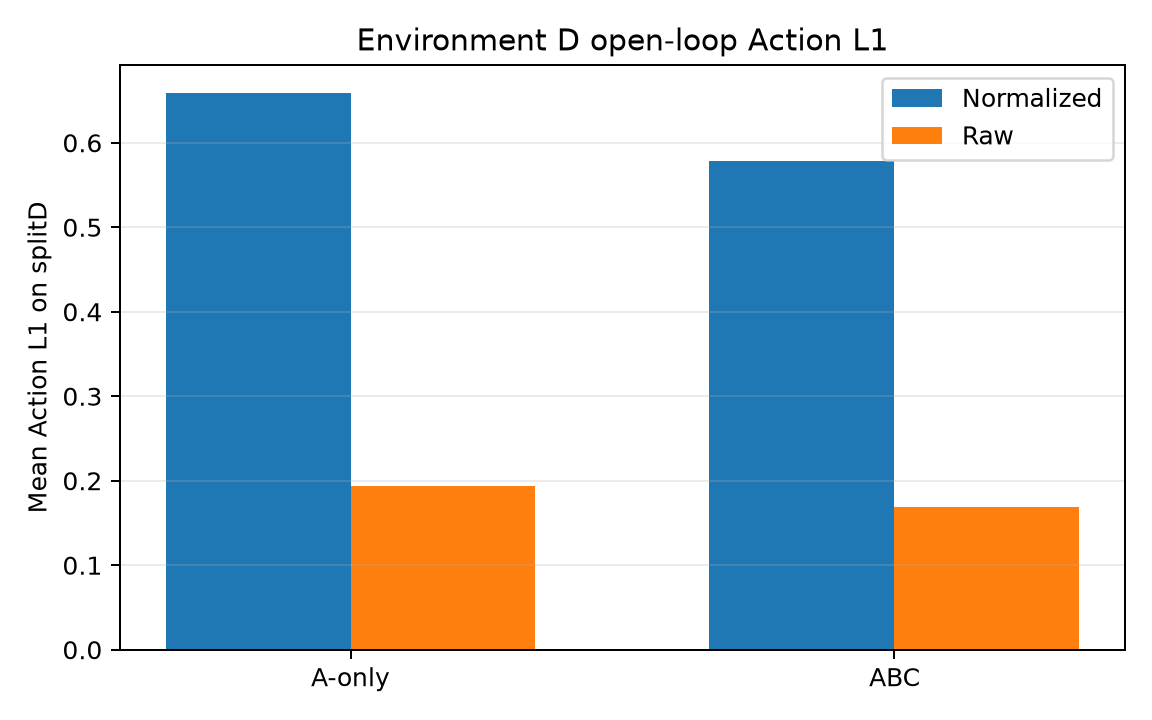
\includegraphics[width=0.72\linewidth]{topic2_splitD_action_l1_bar.png}
  \caption{Environment D open-loop Action L1 comparison in normalized and raw action spaces.}
  \label{fig:topic2-splitd-bar}
\end{figure}

图~\ref{fig:topic2-per-chunk} 展示 chunk 内不同 future-action offset 的误差变化。A-only 的 normalized L1 从前 10 个 offset 的 0.6023 上升到 offset 25--34 的 0.6955，再上升到 offset 55--64 的 0.8246；ABC 的对应数值为 0.5192、0.6236 和 0.7095。最末有效 offset 64 上，A-only 为 0.8331，ABC 为 0.7357。ABC 在所有有效 offset 上保持更低误差，说明额外 B/C 视觉布局提升了环境 D 视觉偏移下的动作预测鲁棒性。

\begin{figure}[h]
  \centering
  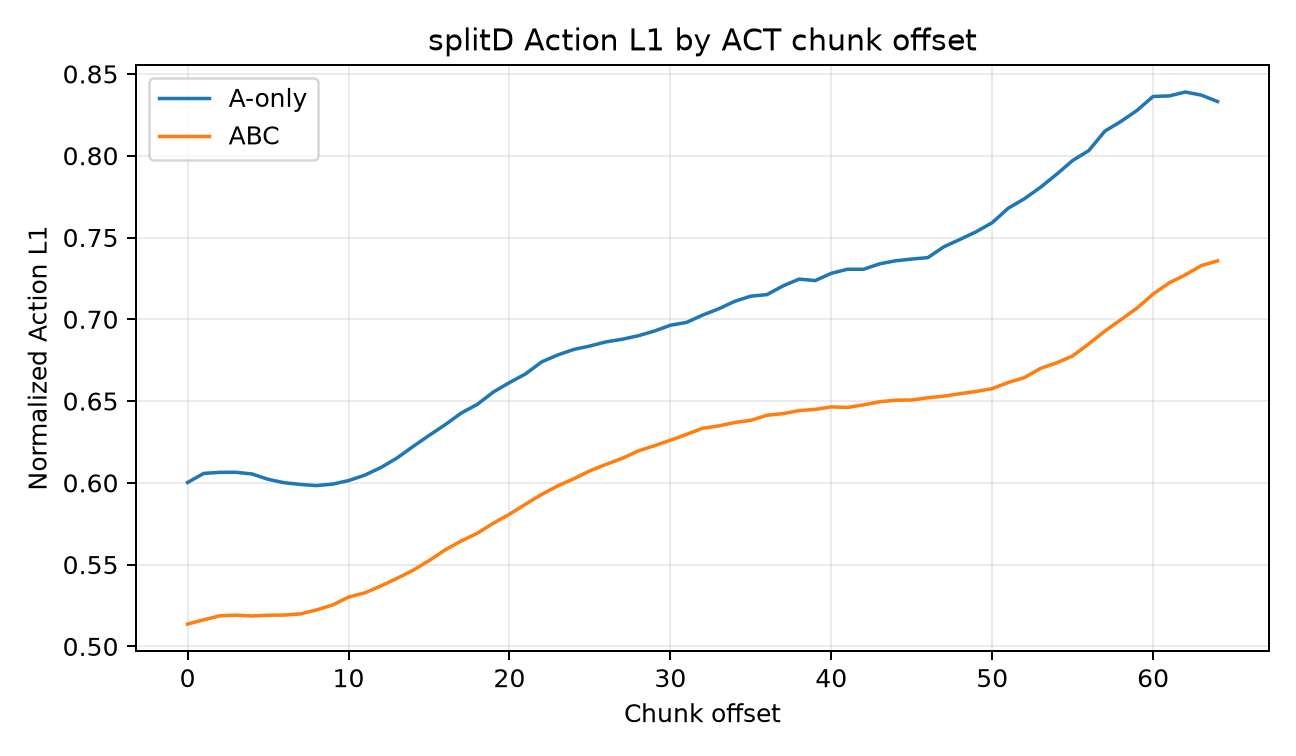
\includegraphics[width=0.82\linewidth]{topic2_splitD_per_chunk_l1.png}
  \caption{splitD normalized Action L1 by ACT chunk offset.}
  \label{fig:topic2-per-chunk}
\end{figure}

帧级误差分布进一步支持上述结论。图~\ref{fig:topic2-error-distribution} 比较 splitD 每帧有效 action chunk mean L1 的分布；两组评测的分布计数都等于 308918 帧。A-only 的帧级 median / p75 / p95 分别为 0.6132 / 0.7888 / 1.0627，ABC 为 0.5211 / 0.7004 / 0.9728；p95 相对降低 8.45\%。结构化统计来自 \path{topic2_act/eval/results/day6_action_chunking_robustness.json}、\path{.csv} 和 \path{.md}。

\begin{figure}[h]
  \centering
  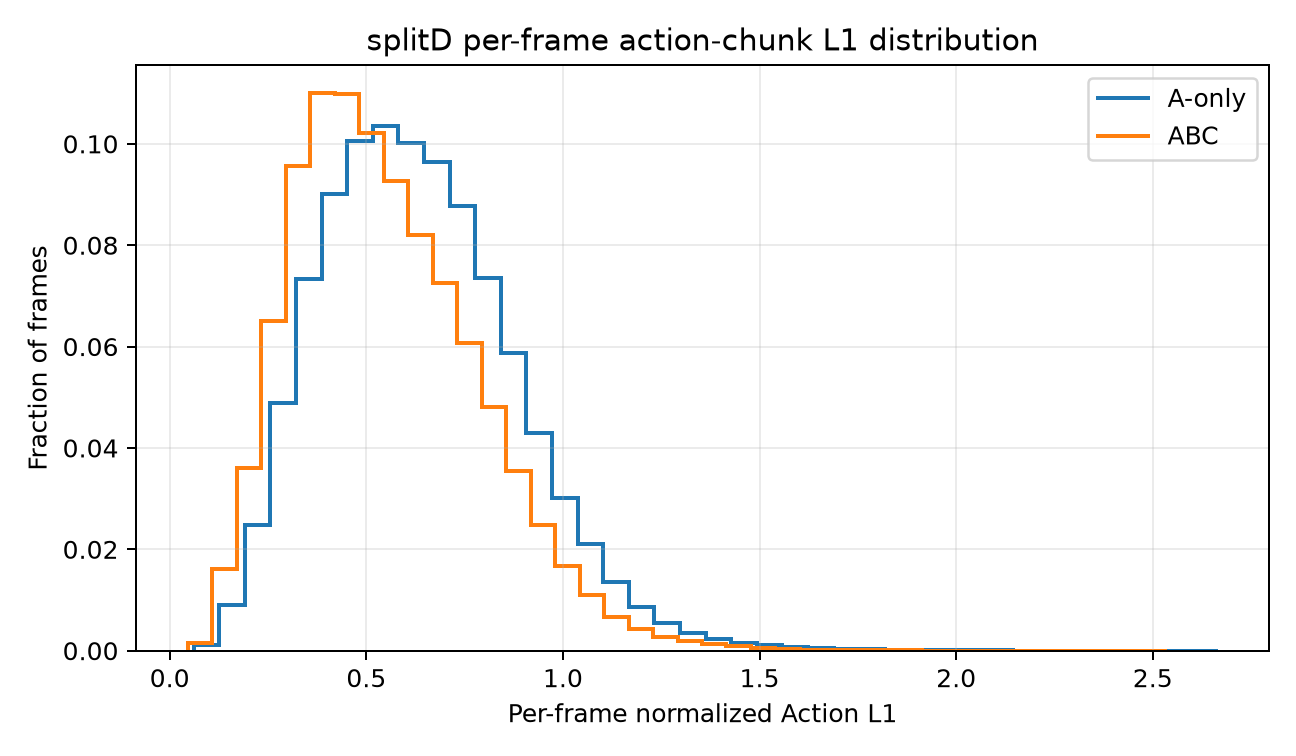
\includegraphics[width=0.82\linewidth]{topic2_splitD_error_distribution.png}
  \caption{splitD per-frame action-chunk mean L1 distribution for A-only and ABC.}
  \label{fig:topic2-error-distribution}
\end{figure}

\section{Discussion}

Topic 1 的结果表明，多来源 3D 资产融合的主要难点集中在表示转换与视觉一致性。真实多视角路线在 PSNR 与物理一致性上更可靠，但从 Gaussian 到 Blender mesh 的转换会引入清理和纹理重建工作；DreamFusion 能快速生成语义明确的物体，但局部几何和纹理稳定性受 prompt、seed 与 SDS 优化影响；Stable Zero123 的采集成本最低，但对输入 crop、alpha matte 和单图视角先验敏感。最终融合视频已经展示了同一相机轨迹下的空间对齐，同时也保留了背景 floater、局部暗部和生成式 mesh 纹理噪声等局限，这些局限应作为三种 3D 资产路线比较的一部分。

Topic 2 的核心现象是训练损失与跨环境泛化并不完全一致。A-only 的最终训练 action L1 低于 ABC，说明单环境训练更容易拟合 splitA 分布；在未见 splitD 上，ABC 的 open-loop Action L1、raw L1、chunk-offset L1 和 frame-level p95 均优于 A-only，说明额外环境覆盖提升了视觉布局变化下的动作预测鲁棒性。比较公平性来自固定训练步数、固定模型结构和固定优化配置。strict EGL 的系统限制使 closed-loop success rate 无法作为主指标；全量 splitD open-loop Action L1 不依赖仿真图形栈，覆盖全部 5124 episodes，因此是本阶段更稳定的主结论依据。

\section{Conclusion}

本阶段完成了 Week4 Day1 的报告骨架收口、前置章节定稿草稿和图表归集。Topic 1 已整理 \texttt{counter}/\texttt{object\_A} contact sheet、hamburger validation/texture、object C training strip/texture、counter orbit 帧和三张融合关键帧；Topic 2 已整理四张训练与评测图，并将 Day6 hyperparameter 与 splitD metric 表写入 LaTeX。当前证据支持两个结论：多来源 3D 融合已经形成可复现工程闭环，但视觉质量受表示转换和生成式资产质量限制；ACT 的多环境 ABC 训练在未见环境 D 上显著优于 A-only，normalized Action L1 相对降低 12.24\%。后续收尾应集中在 README、云盘权重链接、最终 PDF 编译核对和端到端复现记录。

\nocite{*}
\bibliographystyle{plainnat}
\bibliography{reports/references}

\end{document}
